
\documentclass[final]{beamer}



\usepackage[scale=0.8,size=a1]{beamerposter} % Use the beamerposter package for laying out the poster

\usetheme{confposter} % Use the confposter theme supplied with this template
\usepackage{multicol}
\setbeamercolor{block title}{fg=dblue,bg=white} % Colors of the block titles
\setbeamercolor{block body}{fg=black,bg=white} % Colors of the body of blocks
\setbeamercolor{block alerted title}{fg=white,bg=dblue!70} % Colors of the highlighted block titles
\setbeamercolor{block alerted body}{fg=black,bg=dblue!10} % Colors of the body of highlighted blocks
% Many more colors are available for use in beamerthemeconfposter.sty

%-----------------------------------------------------------
% Define the column widths and overall poster size
% To set effective sepwid, onecolwid and twocolwid values, first choose how many columns you want and how much separation you want between columns
% In this template, the separation width chosen is 0.024 of the paper width and a 4-column layout
% onecolwid should therefore be (1-(# of columns+1)*sepwid)/# of columns e.g. (1-(4+1)*0.024)/4 = 0.22
% Set twocolwid to be (2*onecolwid)+sepwid = 0.464
% Set threecolwid to be (3*onecolwid)+2*sepwid = 0.708

\newlength{\sepwid}
\newlength{\onecolwid}
\newlength{\twocolwid}
\newlength{\threecolwid}
\setlength{\paperwidth}{33.1in} % A0 width: 46.8in
\setlength{\paperheight}{23.4in} % A0 height: 33.1in
\setlength{\sepwid}{0.0\paperwidth} % Separation width (white space) between columns
\setlength{\onecolwid}{0.22\paperwidth} % Width of one column
\setlength{\twocolwid}{0.464\paperwidth} % Width of two columns
\setlength{\threecolwid}{0.708\paperwidth} % Width of three columns
\setlength{\topmargin}{-0.5in} % Reduce the top margin size
%-----------------------------------------------------------

\usepackage{graphicx}  % Required for including images

\usepackage{booktabs} % Top and bottom rules for tables
\usepackage{standalone} % to load standalone file (itkz picture for ex)
\usepackage{array} %finest gestion of tabular
\usepackage{algorithm,algorithmicx,algpseudocode}
\usepackage{setspace}

%----------------------------------------------------------------------------------------
%	TITLE SECTION 
%----------------------------------------------------------------------------------------

%\title{Exploring the dynamic of cultural changes: A model to understand the amphorae production patterns in the Roman Empire} % Poster title
%\title{New perspective on the study of variations in Amphorae production during the Roman Empire} % Poster title
\title{Social learning of pottery-making technique\\{\huge An Agent Based Model to understand the amphorae production patterns in the Roman Empire}}

\subtitle{ajsad}

\author{Maria Coto- Sarmiento$^{1,2}$, Simon Carrignon$^{1,3}$ and Xavier Rubio-Campillo$^{1}$} % Author(s)

\institute{$^1$Barcelona Supercomputing Center -- $^2$University of Barcelona -- $^3$Universitat Pompeu Fabra} % Institution(s)

%----------------------------------------------------------------------------------------

\begin{document}

\addtobeamertemplate{block end}{}{\vspace*{2ex}} % White space under blocks
\addtobeamertemplate{block alerted end}{}{\vspace*{2ex}} % White space under highlighted (alert) blocks

\setlength{\belowcaptionskip}{2ex} % White space under figures
\setlength\belowdisplayshortskip{2ex} % White space under equations

\begin{frame}[t] % The whole poster is enclosed in one beamer frame

\begin{columns}[t] % The whole poster consists of three major columns, the second of which is split into two columns twice - the [t] option aligns each column's content to the top

\begin{column}{\sepwid}\end{column} % Empty spacer column

\begin{column}{\onecolwid} % The first column


\begin{block}{Introduction}

\justify

Material culture variability allows us to interpret the change in the production processes~\cite{lycett}. In particular, we want to identify changes on the amphorae production and whether making techniques processes were vertically or horizontally transmitted. A correlation between variation and spatial distance were observed in this study. In this case, amphorae made in nearby workshops might share more similar traits than amphorae made from farthest workshops, following isolation-by distance~\cite{bjo}. If it exists a strong variation on production techniques between workshops correlated with the distance, the learning would be vertical (from master to disciple). Conversely, the learning would be horizontal (learning done by mobile workers with the same level of knowledge). We propose to combine empirical studies with theoretical computer model to test this hypothesis.

\end{block}


\begin{block}{Dataset}

\justify
We analyzed 413 amphorae (fig.\ref{fig:betica}~(b)) from 4 different workshops located in \emph{Baetica} (fig.\ref{fig:betica}~(a)). Amphorae production in this province was really important and active during 300 years in the Roman Empire. The workshops were selected from different sites of \emph{Baetica} province in order to know if morphometric distance was correlated with spatial distance. A set 90 samples from each workshop were used to create a database. 8 measures focused on the rim were taken from each amphorae sample. 

\begin{figure}
\begin{tabular}{cc}


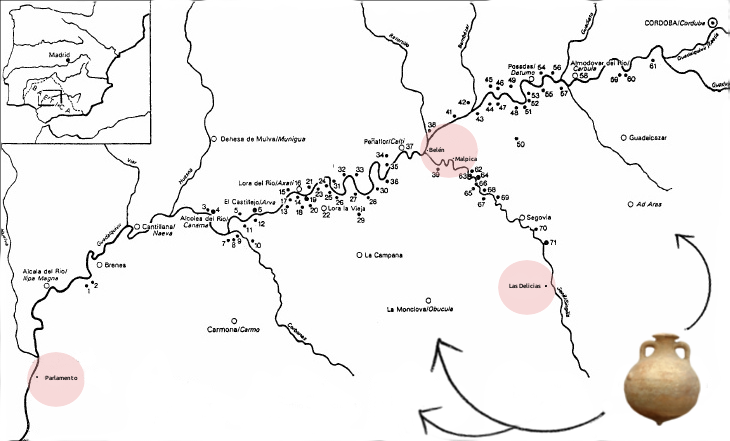
\includegraphics[width=0.7\linewidth]{images/fig1.png} &
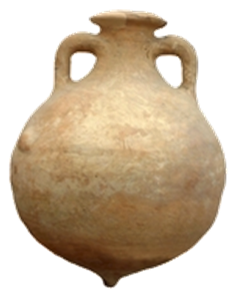
\includegraphics[width=0.2\linewidth]{images/amphorae.png} \\
(a) & (b)
\end{tabular}

\singlespace
\caption{a) More than 80 pottery workshops were distributed along rivers Guadalquivir and Genil. Red circles belong to the workshops analyzed. b) Dressel 20 amphora}
\label{fig:betica}
\end{figure}


 \end{block}
\end{column} % End of the first column

%BEGIN THE SECOND COLUMN-------------------------------------------------
\begin{column}{\twocolwid}


\begin{block}{Empirical Analysis}

\begin{columns}[t,totalwidth=\twocolwid]
\begin{column}{\onecolwid} %first subcolumn left


{\textbf{Principal Component Analysis}} 
\justify

PCA was used to explore these metrical observations with the 8 measurement as variables. Results allow us to simplify the analysis by grouping the variance of the dataset. The first two principal components were chosen to see the significant differences among workshops. 

%\vspace{1cm}

\end{column}

\begin{column}{\sepwid}\end{column} % Empty spacer column

\begin{column}{\onecolwid} %first subcolumn right

{\textbf{Results}}\\
\justify
Figure~\ref{fig:pca} suggests that amphorae from closer workshops tend to be more similar. Most of the workshops have different signals on PC1 (i.e. Bel\'en, Delicias and Malpica) while Parlamento shows a distinctive pattern on PC2.

\end{column}
 % End of the second column
\end{columns}

\begin{columns}[t,totalwidth=\twocolwid]


\begin{column}{\twocolwid} %first subcolumn left
\begin{figure}
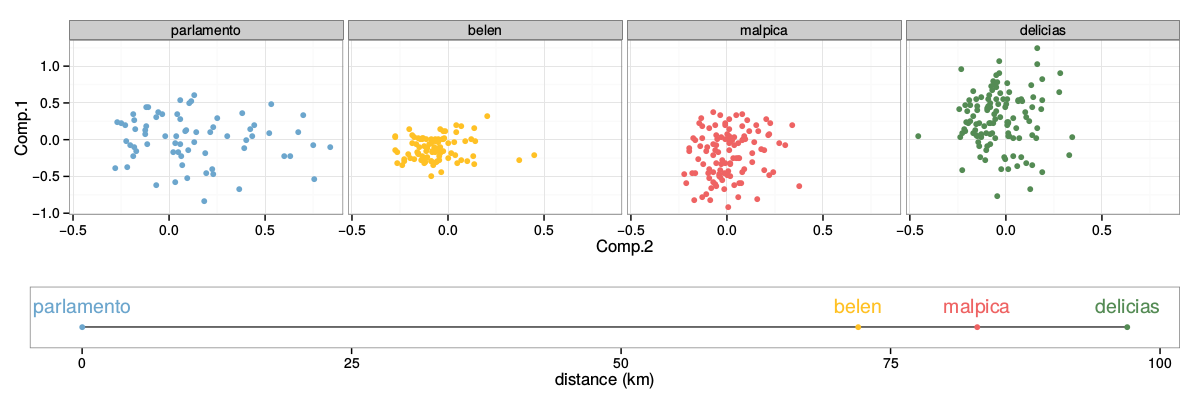
\includegraphics[width=0.6\linewidth]{images/fig2.png}
\singlespace
\caption{First and Second Principal Components for amphorae measured from 4 different workshops}
\label{fig:pca}
\end{figure}
\end{column}
\end{columns}
\end{block}
\vspace{-1cm}
\begin{block}{Theoretical Exploration}

\begin{columns}[t,totalwidth=\twocolwid]

\begin{column}{1.025\onecolwid} %first subcolumn left
%on the left
{\textbf{Model }}
\justify
We propose a model based on classical random drift model \cite{bentley2004randomdriftandculturechange} to test the impact of horizontal vs vertical transmission (HT vs VT) on the variation in production between workshops.  %and to give an idea on which conditions can explain the variation revealed by the PCA. 

A set $Pop$ of $N$ workshops sharing the same initial production technics $P^{0}$ are positioned along a line at increasing distances.% (Fig~\ref{fig:mod},~left). %In this model workshops produce a certain number of amphorae \& can: (1) change their production technics following a random inovation procedure (vertical transmission) or (2) copy the production techniques of another workshop.
 The algorithm is defined as following : %given in the Fig~\ref{fig:mod}~(right).  
%where a fixed number of workshop produce a fixed amount of amphora during a certain time following a certain techniques. Every 100 time step each workshop have a certain probability to slightly modify their production technique (\emph{ie} the vertical tramsission) or to copy the one used by another workshop (\emph{the horizontal transmission}). 
\vspace{.7cm}

	%\begin{figure}
\begin{columns}
%    \begin{column}{.4\textwidth}
	    \centering
%	\resizebox{\textwidth}{!}{
%	    \documentclass{standalone}

\begin{document}
    \begin{tikzpicture}[thick,scale=2]
		\coordinate (WS0) at (0,0);
		\coordinate (WS1) at (1,0);
		\coordinate (WS2) at (2,0);
		\coordinate (WS3) at (3,0);
		\draw[thick,-] (0,0) -- (3,0) node[anchor=north west] {};   
		\foreach \x in {0,1,2,3}
		\draw (\x cm,2pt) -- (\x cm,-2pt) node[anchor=north] {$WS_\x$};


		\draw [black,shorten <= 0.25cm, shorten >= 0.25cm, <->] (WS1) to[out=80,in=100,distance=1cm] node[above,font=\scriptsize]{knowledge transmission} (WS3); 


	\draw [black,shorten <= 0.7cm, shorten >= 0.7cm, <->] (WS0) to[out=-80,in=-100,distance=.75cm	]  node[font=\scriptsize,pos=.60	,above]{$T_{0 \rightarrow 1}$} (WS1);
	\draw [black,shorten <= 0.7cm, shorten >= 0.7cm, <->] (WS0) to[out=-80,in=-100,distance=1cm	]  node[font=\scriptsize,pos=.75	,above]{$T_{0 \rightarrow 2}$}(WS2);
	\draw [black,shorten <= 0.7cm, shorten >= 0.7cm, <->] (WS0) to[out=-80,in=-100,distance=1.25cm	]  node[font=\scriptsize,pos=.82		,above]{$T_{0 \rightarrow 3}$}(WS3);

    \end{tikzpicture}

\end{document}


%}
%    \end{column}
    \begin{column}{.9\textwidth}
	\begin{algorithm}[H]
	    \begin{algorithmic}
		\footnotesize
		\State INITIALIZATION:
		\For{$i \in Pop$}
		\State $P^{i} = P^{0}$
		\EndFor
		\State SIMULATION:
		\Loop{$~step \in TimeSteps$}
		\For{$i \in Pop$}
		\State $AmphoraProduction(P^{i})$
		\If{$ (step \mod 100) = 0$}	
		\State $P^{i}=Innovation(P^{i})$ \Comment{Vertical Transmission}
		\State $P^{i}=RandomCopy(Pop)$	\Comment{Horizontal Transmission}
		\EndIf
		\EndFor
		\EndLoop
	    \end{algorithmic}
	    %\caption{Schema (left) and pseudo-code (right) of the model }
	    \caption{Model }
	    \label{fig:mod}
	\end{algorithm}
   \end{column}
\end{columns}

%\singlespace

%{\textbf{Horizontal Transmission}}\\




\end{column}

%\begin{column}{.2\sepwid}\end{column} % Empty spacer column

\begin{column}{1.025\onecolwid} %first subcolumn right
{\textbf{Experiment \& Result}}\\
\justify
We simplify the problem by focusing on the variation of one trait. To measure the influence of HT \& spatial distance we bias the random copy toward the closest neighbour. We define $P(T_{AB})$ the probability that $WS_A$ copy $WS_B$ as $\frac{1}{f(d)}$, where $d$ is the distance between $A$ and $B$.
For each level of bias we run $100$ simulations with 4 workshops and we look how the trait varies between each workshop at the end.

The fig~\ref{fig:resmod} shows that variation in production is high only if there is no HT or if the transfer is strongly biased toward the closest neighbour.
\vspace{-1cm}

    \begin{figure}[h!]
    \centering
	%\begin{tabular}{m{.3\textwidth}m{.3\textwidth}m{.3\textwidth}}
%    \begin{tabular}{ccc}
%	     $f(d)=d$ & $f(d)=d^3$ & No Copy\\
%	    
%	    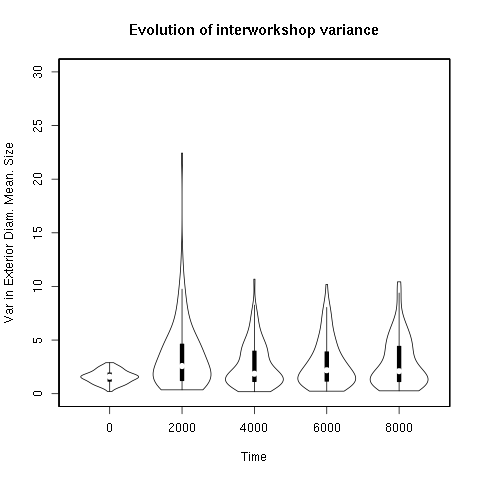
\includegraphics[height=.3\textwidth]{images/lineC.png}
%	    &
%	    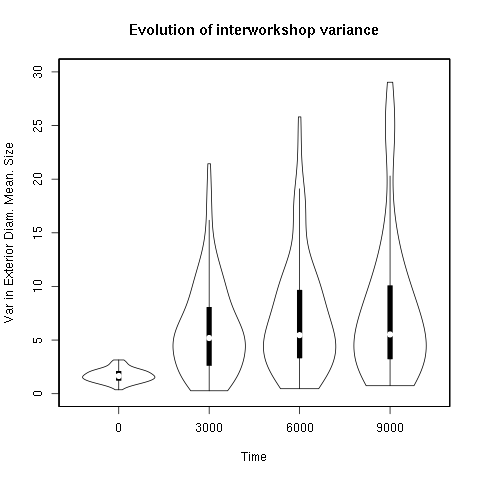
\includegraphics[height=.3\textwidth]{images/cubeC.png}
%	    &
%	    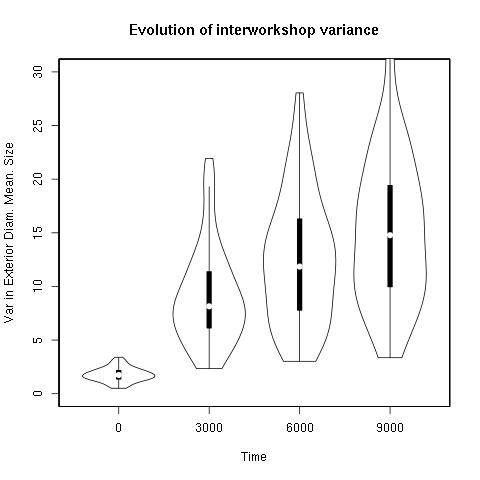
\includegraphics[height=.3\textwidth]{images/lineNC.png}\\
%	\end{tabular}
	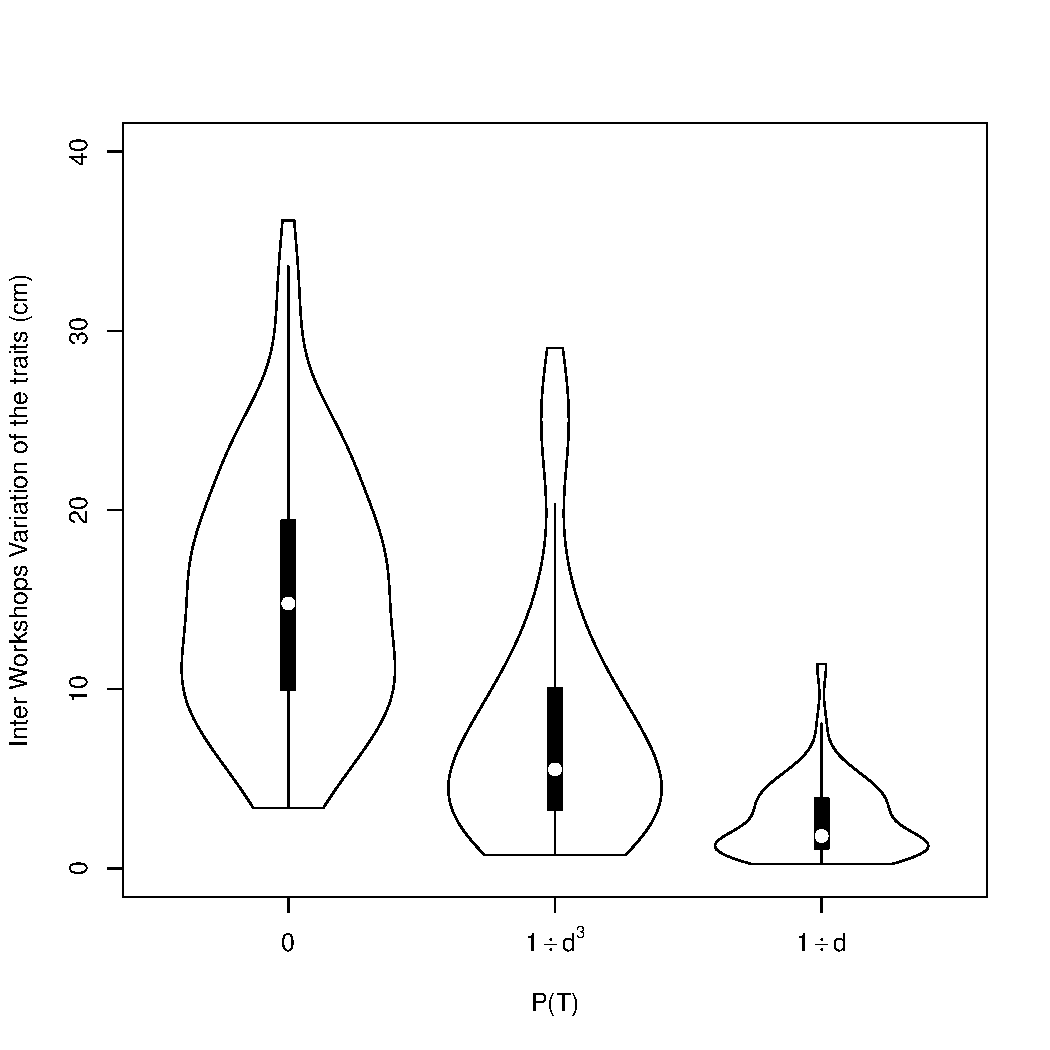
\includegraphics[width=0.5\linewidth]{images/interworkshopvar.pdf}
\singlespace
\vspace{-.8cm}
\caption{Inter-workshop variation of the mean of the trait after $10\,000$ timestep in setup where the horizontal transfer probability varies (100 simulations per condition).}
	\label{fig:resmod}
    \end{figure}
\vspace{-1cm}



    
\end{column}
 % End of the second column
\end{columns}

\end{block}
\end{column}

%BEGIN LAST COLUMN----------------------------------------------------

%\begin{column}{\sepwid}\end{column} % Empty spacer column

\begin{column}{\onecolwid} % The third column

\begin{block}{Discussion}
\justify

Empirical studies has identified variation on the making techniques processes among pottery workshops. We observe that this variability is affected by the distance: amphorae made in nearby workshops with a minor spacial distance share more similar traits than amphorae made in pottery workshops farther. It suggests that the pottery techniques were learned from master to disciple instead of workers with the same level. 

The combination of this empirical analysis with the theoretical model suggests that horizontal transmission could not be the main cultural process in the workshops. This result, combined with the correlation between spatial distance and morphometric distance suggests that vertical transmission is probably the most probable mechanism.


%This is still  preliminary results as both empirical and theoretical analysis need to be improved: each one using the result of the other. 

%the first on by collecting more data from other sites to see if the inter-workshop variation is still consistent with isolation by distance ; the second one by bringing closer the model to the case study by make co-variate as variable as in the empirical study and by integrating the observed correlation between the variable.  
 
\end{block}

\begin{block}{References}
\small

\begin{thebibliography}{50}


\bibitem[1]{lycett}\textsc{Lycett, S.J (2015)}
\textit{Cultural evolutionary approaches to artifact variation over time and space: basis, progress, and prospects}, Journal of Archaeological Science, 56, 21-31.

\bibitem[2]{bjo}\textsc{Bj\"{o}rklund, M., Bergek, S., Ranta, E., \& Kaitala, V. (2010)}
\textit{The effect of local population dynamics on patterns of isolation by distance}, Ecological Informatics, 5(3), 167-172.

\bibitem[3]{bentley2004randomdriftandculturechange}\textsc{Bentley, R., Hahn, M., Shennan, S. (2004)}
\textit{Random drift and culture change}, Proceedings of the Royal Society of London. Series B: Biological Sciences, 271(1547), 1443--1450.


\end{thebibliography}
%	\scriptsize
%	\renewcommand{\refname}{\vspace{-0.5em}}
%	//\bibliographystyle{abbrv}
%	\bibliography{biblio}

\end{block}

%----------------------------------------------------------------------------------------
%	ACKNOWLEDGEMENTS
%----------------------------------------------------------------------------------------

\setbeamercolor{block title}{fg=dblue,bg=white} % Change the block title color

\begin{block}{Acknowledgements}

\small{\rmfamily{The Funding for this work was provided by the ERC Advanced Grant EPNet (340828).}}

\end{block}

%----------------------------------------------------------------------------------------
%	CONTACT INFORMATION
%----------------------------------------------------------------------------------------

\setbeamercolor{block alerted title}{fg=white,bg=dblue!70} % Change the alert block title colors
\setbeamercolor{block alerted body}{fg=black,bg=white} % Change the alert block body colors


\begin{center}
\begin{tabular}{ccc}

\includegraphics[width=0.52\linewidth]{images/epnet.png} & \hfill & 
\includegraphics[width=0.5\linewidth]{images/erc.png}
\end{tabular}
\end{center}

%----------------------------------------------------------------------------------------

\end{column} % End of the third column

\end{columns} % End of all the columns in the poster

\end{frame} % End of the enclosing frame

\end{document}
